%% V1.0
%% by Gabriel Garcia, gabrcg@gmail.com
%% This is a template for Udacity projects using IEEEtran.cls

%% Be Udacious!

\documentclass[10pt,journal,compsoc]{IEEEtran}

\usepackage[pdftex]{graphicx}    
\usepackage{cite}
\usepackage[inline]{enumitem}
\usepackage{subfigure}
\usepackage{hyperref}
\usepackage{algorithmic}
\usepackage{algorithm}
\hyphenation{op-tical net-works semi-conduc-tor}


\begin{document}

\title{Map My World Robot}

\author{Saminda Abeyruwan}

\markboth{Inference project, Robotic Nanodegree, Udacity}%
{}
\IEEEtitleabstractindextext{%

\begin{abstract}
Simultaneous Localization and Mapping (SLAM), a robot acquires a map of the environment and simultaneously localize itself relative to the map. Each robot platform contains a set of constraints on sensors, locomotion, and compute power,  SLAM approaches that address these constraints provide real-time  benefits to practitioners.  Real-Time Appearance-Based Mapping (RTAB-Map) is a an open source loop closure detection with memory management library that addresses these limitations for long-term and large scale environment mapping. This project evaluates RTAB-Map 2D and 3D mapping and localization modalities in two Gazebo environments using a RGB-D camera mounted on a four-wheeled robot.  
%An abstract is meant to be a summary of all of the relevant points in your presented work. It is designed to present a high-level overview of the report, providing just enough detail to convey the necessary information The abstract may often mention a one-sentence summary of the results.  While the type of voice chosen for the paper (active or passive) may be up for debate, you should avoid the use of “I” and “me” in the report. It usually is kept to a length of 150 - 200 words. 
%Example: You should not write, “I present two different neural networks for classifying my data”. Instead, you should try to say, “Two different neural networks are used for classification”.
\end{abstract}

% Note that keywords are not normally used for peerreview papers.
\begin{IEEEkeywords}
Robot, IEEEtran, Udacity, \LaTeX, RTAB-Map.
\end{IEEEkeywords}}


\maketitle
\IEEEdisplaynontitleabstractindextext
\IEEEpeerreviewmaketitle
\section{Introduction}
\label{sec:introduction}

\IEEEPARstart{O}{ne} of the fundamental problems inherent to an autonomous robots is to identify an unknown environment and localize itself relative to it, which has been known as the Simultaneous Localization and Mapping (SLAM) problem \cite{Thrun:2005:PR:1121596}.  Unlike the localization problem, the robot must infer the map and its location from the measurements $z_{1:t}$ and controls $u_{1:t}$.  In addition, SLAM must address constraints impose by sensors, locomotion, compute power, cost, accuracy, integration, and real-time requirements of the applications. 

Real-Time Appearance-Based Mapping (RTAB-Map) \cite{Labbe:2018} is an open source library that implements loop closure detection with a memory management approach that addresses the prior constraints and able to use long-term and large-scale environment mapping. RTAB-Map provides online processing, robust under low-drift odometry, robust localization, practical map generation and exploitation, and multi-session mapping. 

This project leverages RTAB-Map implementation available in the Robotic Operating Systems (ROS) \cite{288} to map two Gazebo environments. A four-wheeled robot (developed in the localization project) mounted  with a RGB-D camera has been used to map the environments, and localize itself relative to the the databases constructed from the RTAB-Map packages.    

\begin{figure}[thpb]
      \centering
      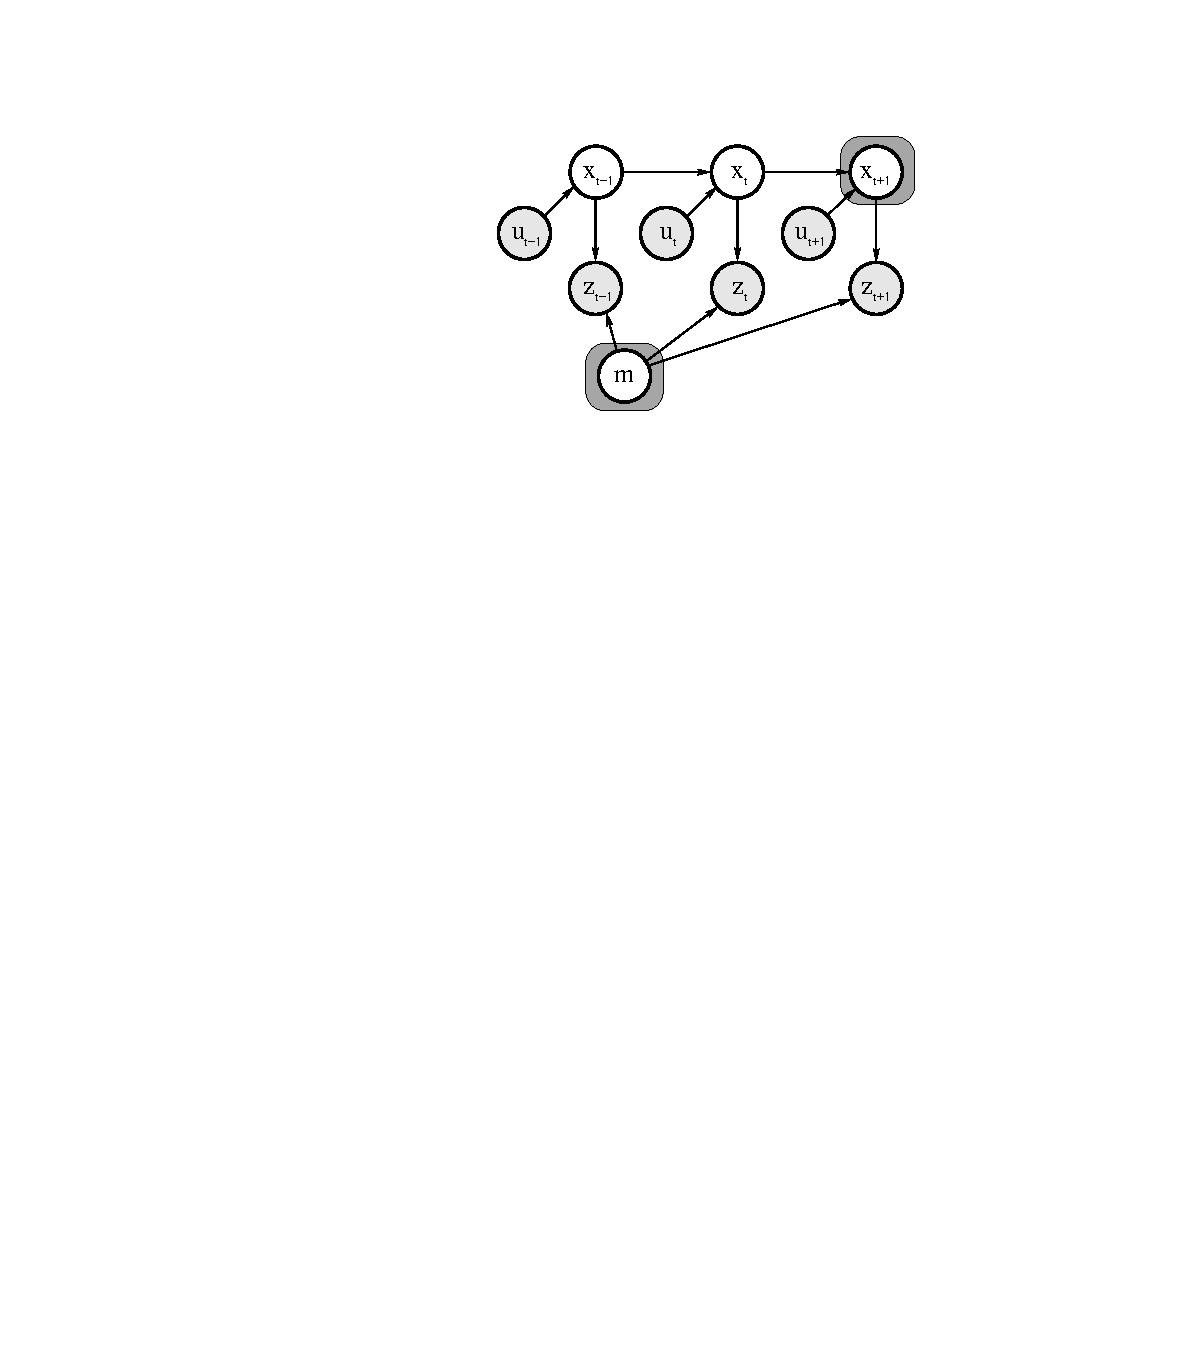
\includegraphics[width=\linewidth]{online_slam}
      \caption{Graphical model of the online SLAM problem. The orignal figure is available in\cite{Thrun:2005:PR:1121596} (Figure 10.1).}
      \label{fig:online_slam}
\end{figure}
 
%introduction should provide some material regarding the history of the problem, why it is important and what is intended to be achieved. If there exists any previous attempts to solve this problem, this is a great place to note these while conveying the differences in your approach (if any). The intent is to provide enough information for the reader to understand why this problem is interesting and setting up the conversation for the solution you have provided
%Use this space to introduce your robotic inference idea and how you wish to apply it. 
%If you have any papers / sites you have referenced for your idea, please make sure to cite them.

%example for inserting image
%\begin{figure}[thpb]
%      \centering
%      \includegraphics[width=\linewidth]{RobotRevolution5}
%      \caption{Robot Revolution.}
%      \label{fig:robot1}
%\end{figure}

%\subsection{Subsection Heading Here}
%Subsection text here.
%
%\subsubsection{Subsubsection Heading Here}
%Subsubsection text here.
%
%
%\begin{table}[h]
%\caption{Table}
%\label{table_example}
%\begin{center}
%\begin{tabular}{|c||c|}
%\hline
%One & Two\\
%\hline
%Three & Four\\
%\hline
%\end{tabular}
%\end{center}
%\end{table}



   

\section{Background}

There are two versions of the SLAM problem. The first is known as \textit{online SLAM}, which estimates the pose, $x_t$ at time $t$ and map $m$, given the measurements  $z_{1:t}$ and controls $u_{1:t}$., $p(x_t, m | z_{1:t}, u_{1:t})$. The graphical model of the online SLAM problem is shown in Fig. \ref{fig:online_slam}. This method evaluates variables at time $t$, it is incremental, and discard past measurement and controls once they have been processed.  The second SLAM problem is known as \textit{full SLAM}, which estimates posterior over the entire path $x_{1:t}$ and the map $m$, $p(x_{1:t}, m | z_{1:t}, u_{1:t})$. The online SLAM problem is the result of integrating all the variables past time $t$ of the full SLAM problem, i.e., $p(x_t, m | z_{1:t}, u_{1:t}) = \int \int \dots \int p(x_{1:t}, m | z_{1:t}, u_{1:t}) dx_1 dx_2 \dots dx_{t-1}$. The graphical model of the full SLAM problem is shown in Fig. \ref{fig:full_slam}. There are several popular SLAM algorithms: 

\begin{figure}[thpb]
      \centering
      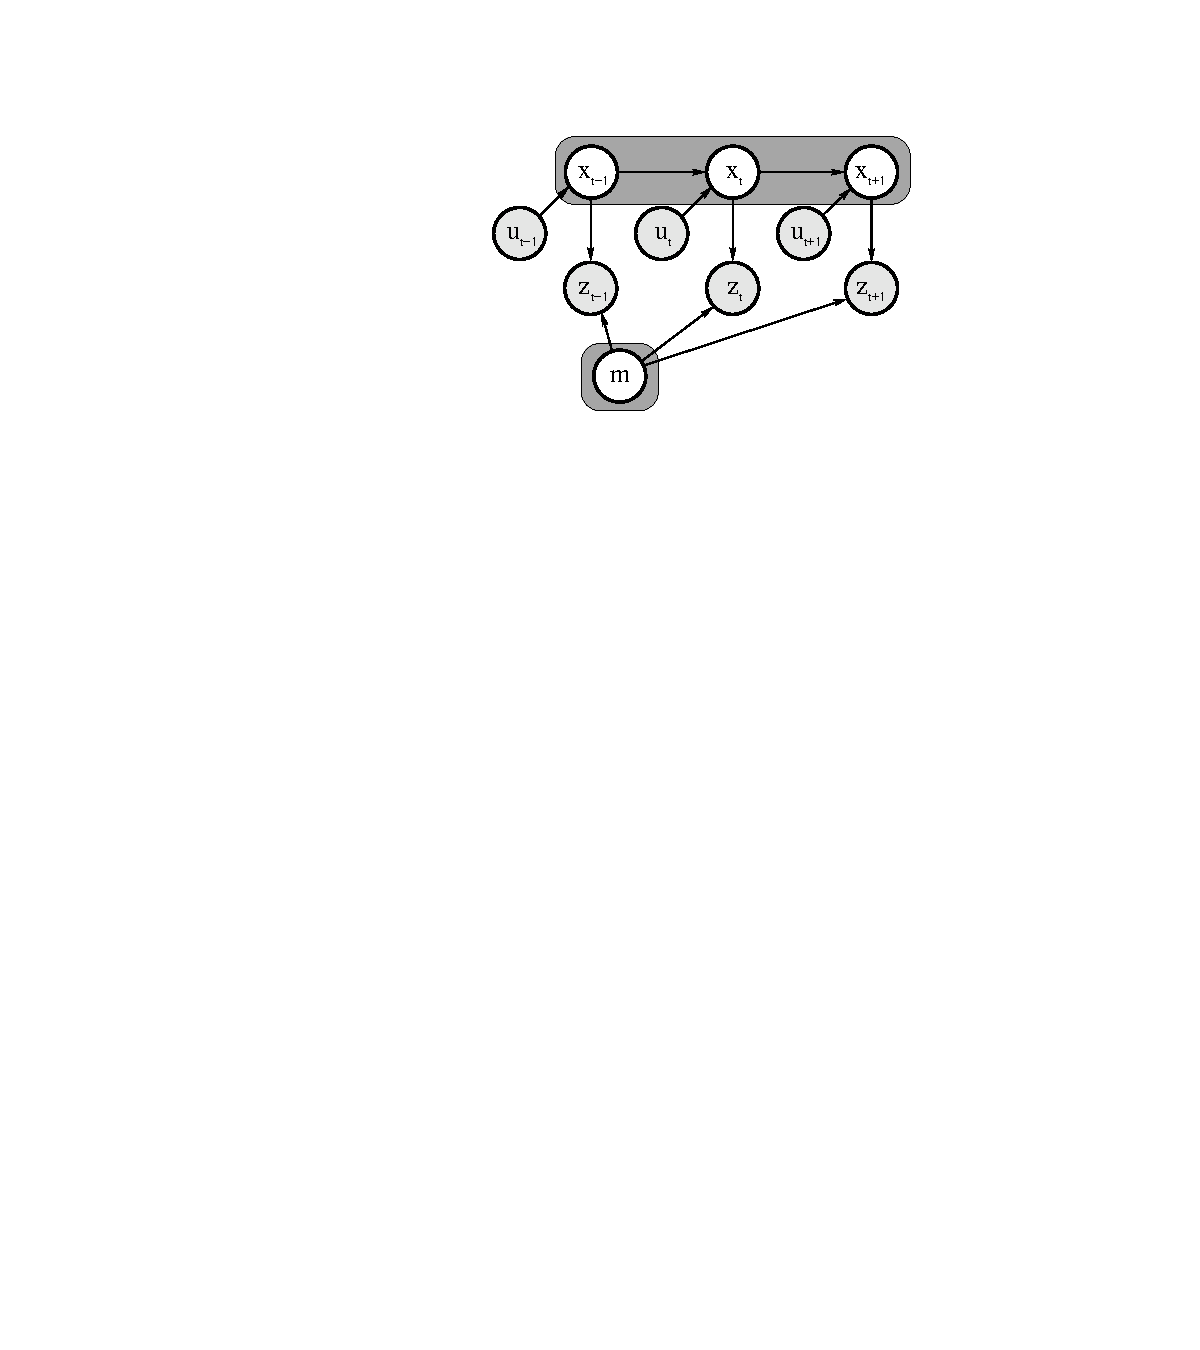
\includegraphics[width=\linewidth]{full_slam}
      \caption{Graphical model of the full SLAM problem. The orignal figure is available in\cite{Thrun:2005:PR:1121596} (Figure 10.2).}
      \label{fig:full_slam}
\end{figure}

\begin{enumerate} \item SLAM with extended Kalman filter: which applied the EKF to online SLAM using maximum likelihood data association. The map is feature based and the landmarks are usually limited, and requires significant efforts to detect features. With known correspondence, the updates are time quadratic in the number of landmarks in the map.  \item The GraphSLAM algorithm: which addresses the full SLAM problem. It calculates posterior over full robot path and map, thus, it is a batch algorithm. GraphSLAM constructs a graph of soft constraints, i.e., measurement are mapped into edges that represent nonlinear constraints between poses and sensed features, while motion commands are mapped into soft constraints between consecutive poses. The graph is sparse, and maximizing the sum of the constraints via maximum likelihood estimates the robot path and the map.  \item The sparse extended information filter (SEIF): which is similar to GraphSLAM, however, it integrates out past poses, which resulted in an online SLAM. This is an efficient with information representation and integrating out past poses. To achieve online SLAM, SEIF makes number of approximations, which results in less accurate that GraphSLAM or the EKF.  \item The FastLAM algorithm: is a particle filter approach to SLAM problem. FastSLAM maintains a set of particles, which contains a sampled robot path. It also contains a map, where each feature of the map is represented by it own local Gaussian. This representation requires space linear in the size of the map, and linear in the number of particles. The update in the algorithm follows the conventional particle filter, and updates are preformed online, thus, it solves the online SLAM problem (for further discussion, please refer to chapters 11, 12, and 13 in reference \cite{Thrun:2005:PR:1121596}.\end{enumerate} 

This project uses RTAB-Map, an open source loop closure detection with memory management, is a graph-based SLAM approach that has been integrated to ROS as the  \textit{rtabmap\_ros}. Fig. \ref{fig:rtabmap_ros} shows the block diagram of rtabmap ROS node.  A RGD-B camera, odometry, and laser scan has been used as the external inputs to RTAB-Map. The ROS package, \textit{depthimage\_to\_laserscan} has been used to obtain the laser scan from RGB-D camera.  

RTAB-MAP, structure of the map is a graph with linked nodes. After sensor synchronization, the short-term memory (STM) creates a node memorizing the odometry pose, and additional sensor data, e.g., visual words for loop closure and proximity detection, and local occupancy grid for global map assembly. Nodes are created at a fixed rate (how much data created from nodes overlap each other). Links are added in the STM between consecutive nodes with odometry transformation. Loop closure and proximity links are added through loop closure detection or proximity detection. All the links are used as constraints for graph optimization. When there is a new loop closure or proximity link added to the graph, graph optimization propagates the computed error to the whole graph, to decrease odometry drift. With the graph optimized, OctoMap, and 2D occupancy grid outputs are assembled and published to external packages. RTAB-Map memory management runs on top of the graph, which limits the size of the graph such that long-term online SLAM is achieved in large environment. This is implemented via a working memory (WM) and a long-term memory (LTM). More information about the operations, please refer to \cite{labbertab}.

\begin{figure*}[thpb]
      \centering
      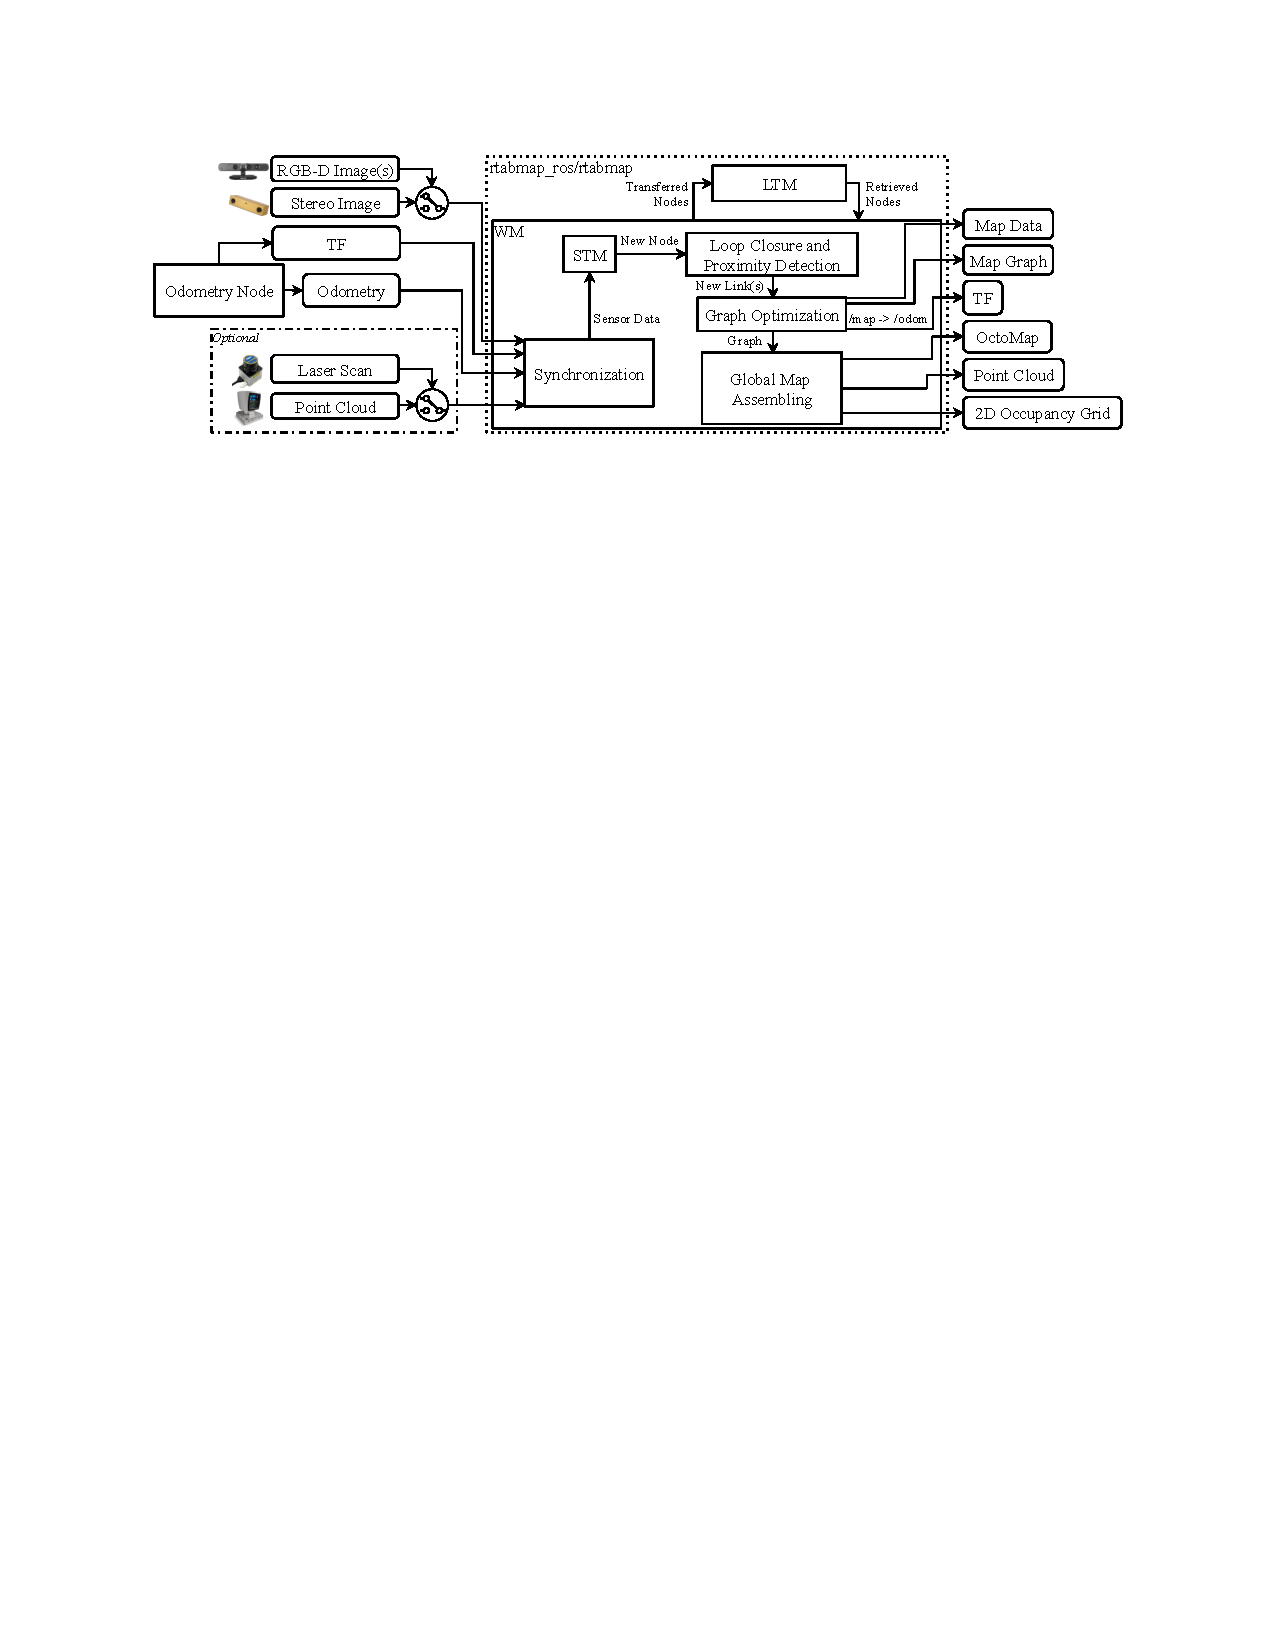
\includegraphics[width=\linewidth]{rtabmap_ros}
      \caption{Block diagram of \textit{rtabmap\_ros}  node. The orignal figure is available in \cite{labbertab} (Figure 1).}
      \label{fig:rtabmap_ros}
\end{figure*}


%\texttt{•}
%At this stage, you should begin diving into the technical details of your approach by explaining to the reader how parameters were defined, what type of network was chosen, and the reasons these items were performed. This should be factual and authoritative, meaning you should not use language such as “I think this will work” or “Maybe a network with this architecture is better..”. Instead, focus on items similar to, ”A 3-layer network architecture was chosen with X, Y, and Z parameters” 
%Explain why you chose the network you did for the supplied data set and then why you chose the network used for your robotic inference project. \cite{Thrun:2005:PR:1121596}
%
%%example for Bullet point list
%
%\begin{itemize}
%\item example
%\end {itemize}
%
%
%
%%example for numbered list
%\begin{enumerate}
%\item example
%
%\end{enumerate}

\section{Scene and Robot Configuration}
%This section should discuss the data set. Items to include are the number of images, size of the images, the types of images (RGB, Grayscale, etc.), how these images were collected (including the method). Providing this information is critical if anyone would like to replicate your results. After all, the intent of reports such as these are to convey information and build upon ideas so you want to ensure others can validate your process.
%Justifying why you gathered data in this way is a helpful point, but sometimes this may be omitted here if the problem has been stated clearly in the introduction.
%It is a great idea here to have at least one or two images showing what your data looks like for the reader to visualize.

\section{Results}
%This is typically the hardest part of the report for many. You want to convey your results in an unbiased fashion. If you results are good, you can objectively note this. Similarly, you may do this if they are bad as well. You do not want to justify your results here with discussion; this is a topic for the next session. 
%Present the results of your robotics project model and the model you used for the supplied data with the appropriate accuracy and inference time
%For demonstrating your results, it is incredibly useful to have some charts, tables, and/or graphs for the reader to review. This makes ingesting the information quicker and easier.

\section{Discussion}
%This is the only section of the report where you may include your opinion. However, make sure your opinion is based on facts. If your results are poor, make mention of what may be the underlying issues. If the results are good, why do you think this is the case? Again, avoid writing in the first person (i.e. Do not use words like “I” or “me”). If you really find yourself struggling to avoid the word “I” or “me”; sometimes, this can be avoid with the use of the word “one”. As an example: instead of : “I think the accuracy on my dataset is low because the images are too small to show the necessary detail” try: “one may believe the accuracy on the dataset is low because the images are too small to show the necessary detail”. They say the same thing, but the second avoids the first person. 
%Reflect on which is more important, inference time or accuracy, in regards to your robotic inference project.

\section{Conclusion / Future work}
%This section is intended to summarize your report. Your summary should include a recap of the results, did this project achieve what you attempted, and is this a commercially viable product? 
%For Future work,address areas of work that you may not have addressed in your report as possible next steps. For future work, this could be due to time constraints, lack of currently developed methods / technology, and areas of application outside of your current implementation. Again, avoid the use of the first-person.

\bibliography{bib}
\bibliographystyle{ieeetr}

\end{document}